\section{Prototypes}
There were used different prototypes to decide, how this program should interact with the user and how the user interface should look like in the end. In this section three different prototypes will be shown and the work process and decision making will be explained.
The first prototypes were drawings on a blackboard or a piece of paper but later we also had an HTML prototype. In this process 2-3 group members made the first design and the presented it to the group which when came with point of improvements which then was discussed and then a new prototype was made until the design was satisfactory.  One of the prototypes, made in HTML, was also shown to the kindergarten teacher Kristine ....who then???...%kommer n�r jeg har h�rt interview

\subsection{The first prototypes}
After the first prototype was presented each page was drawn on to the blackboard where the changes easier were added. One of the first blackboard designs of the page change settings of a child which is e.g. the child's name and abilities is shown in Figure \vref{fig:firstProto}. This is a primitive design with two menus one horizontal and one vertical, where the horizontal has all children and groups of children and the vertical has all the applications on a child's device the user can administer. This menu will be further explained for the next prototype. 

\begin{figure}[ht]
	\centering
		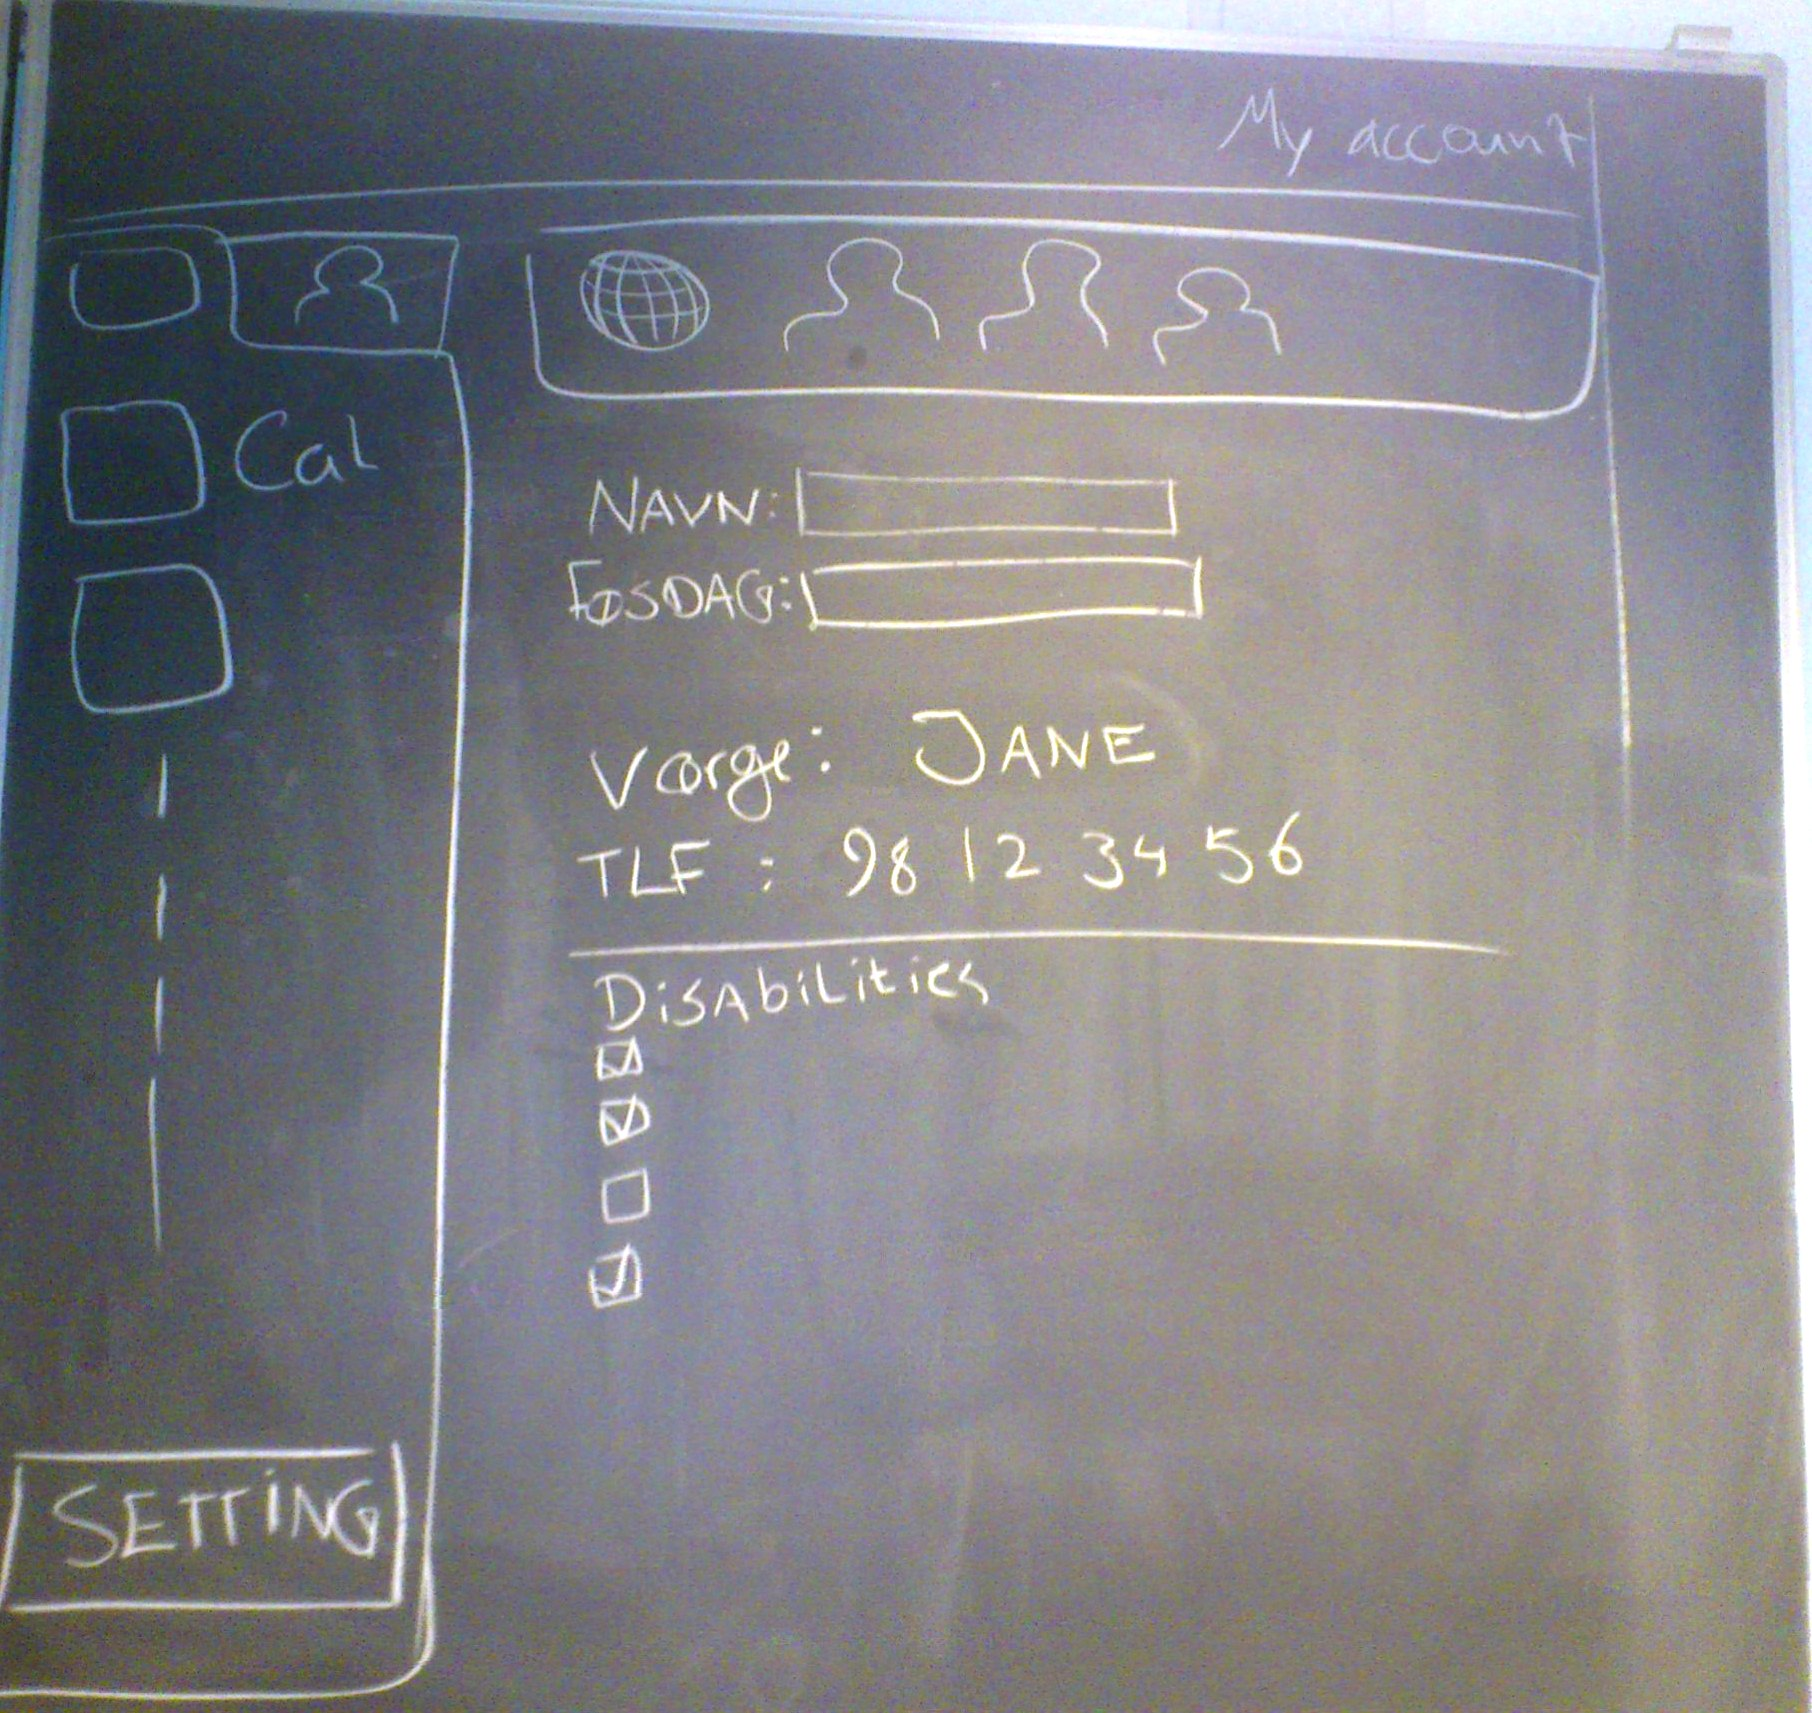
\includegraphics[width=1.00\textwidth]{img/firstproto.jpg}
	\caption{?Changes made on the black board?}
	\label{fig:firstProto}
\end{figure}


The group members did disagree how to get into this page, because in this design the user would have to choose a child in the top horizontal menu and the press the Setting button in the vertical menu, which is located among Giraf application that is to be administrator. Especially the location and the naming of the Setting button were discussed because the user would get the impression that they administer their child like the applications and not changes the information about the child. To solve this it was suggested that this page should be in My Account instead; where the user also would be able to change they own personal information. In our prototypes this was not change until the implementation. ?????not sure????% sp�rg johannes eller se n�r den er f�rdig

\subsection{The HTML prototype}
For the second interview with Kristine an HTML prototype was made from the primitive prototypes. The Figure \vref{fig:contactbook} is two screen shoots from the child Jack's contact book where the right side of the figure is an Light box with an entry from the contact book. The contact book is inspired by a calendar, because for a date it can have some entries that the user can click on and then within a Light box the message and pictures is shown. If the user has not seen the message before, the signal "Ny!" in the right side should be visible. The user is able to fold and unfold the entries for each date, to see or hide the entries in the contact book. 

\begin{figure}[ht]
	\centering
		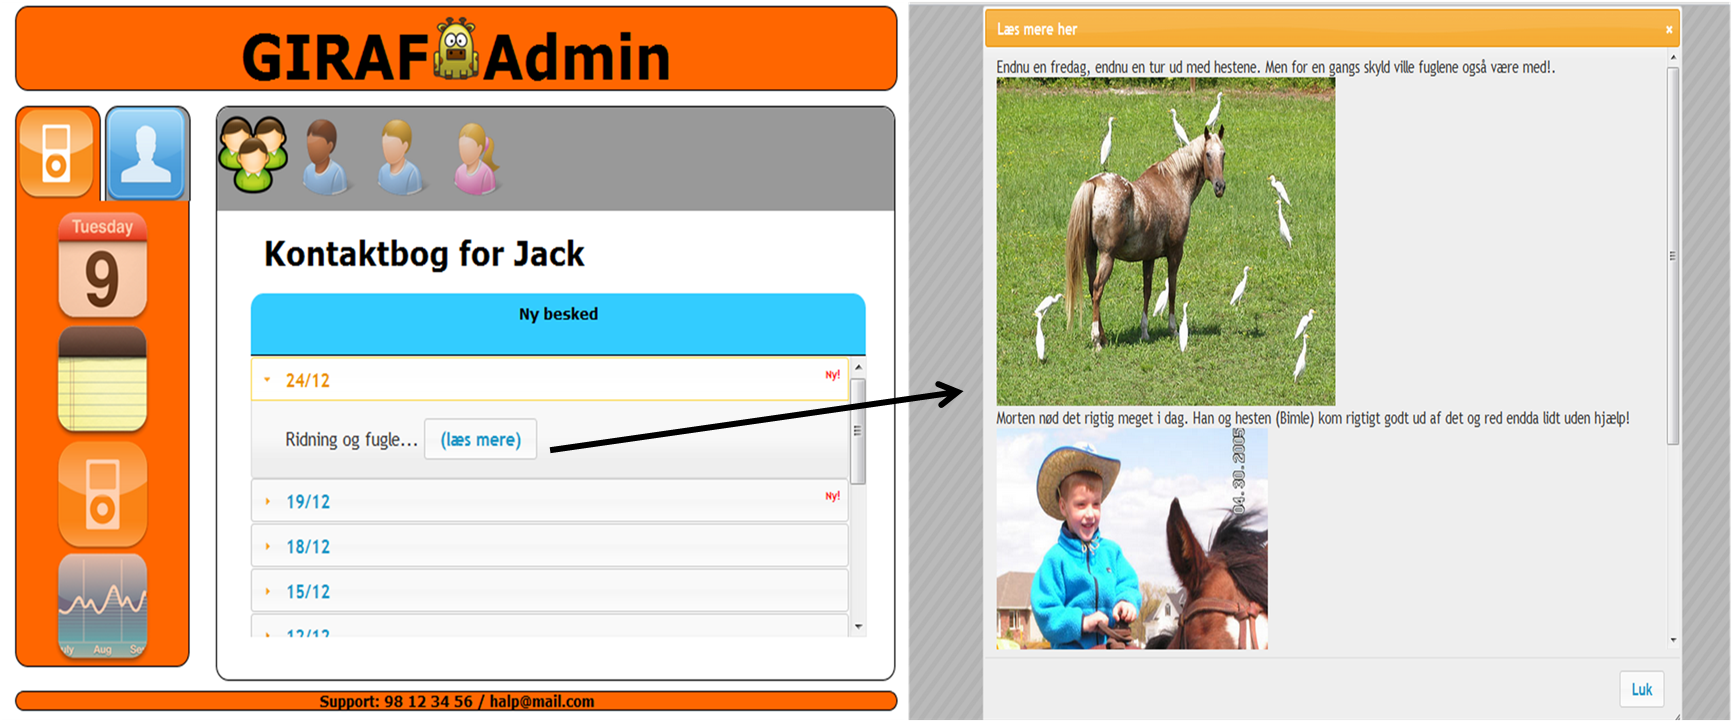
\includegraphics[width=1.00\textwidth]{img/contactbook.png}
	\caption{screenshots from the html prototype}
	\label{fig:contactbook}
\end{figure}

\subsubsection{}
As shown in Figure \vref{fig:contactbook} the Giraf applications' administrators is represented on the vertical menu, as an icon that should identify the application administrator. The children's devices are represented on the horizontal menu where the single child's device is identified from a picture and the group is identified by an icon representing a group of children. However this representation can be mirrored such that the children's devices are represented on the vertical menu and the applications are represented on the horizontal menu, which is shown in Figure \vref{fig:menus}. The black circle indicates which of the menus is represented in the vertical menu. This menu was not implemented because it would take too much of the space on the screen, and it could also be a confusing navigation path for the user, without gaining any new functionality. In the next paper prototype this menu was replaced with two vertical menus side by side.

\begin{figure}[ht]
	\centering
		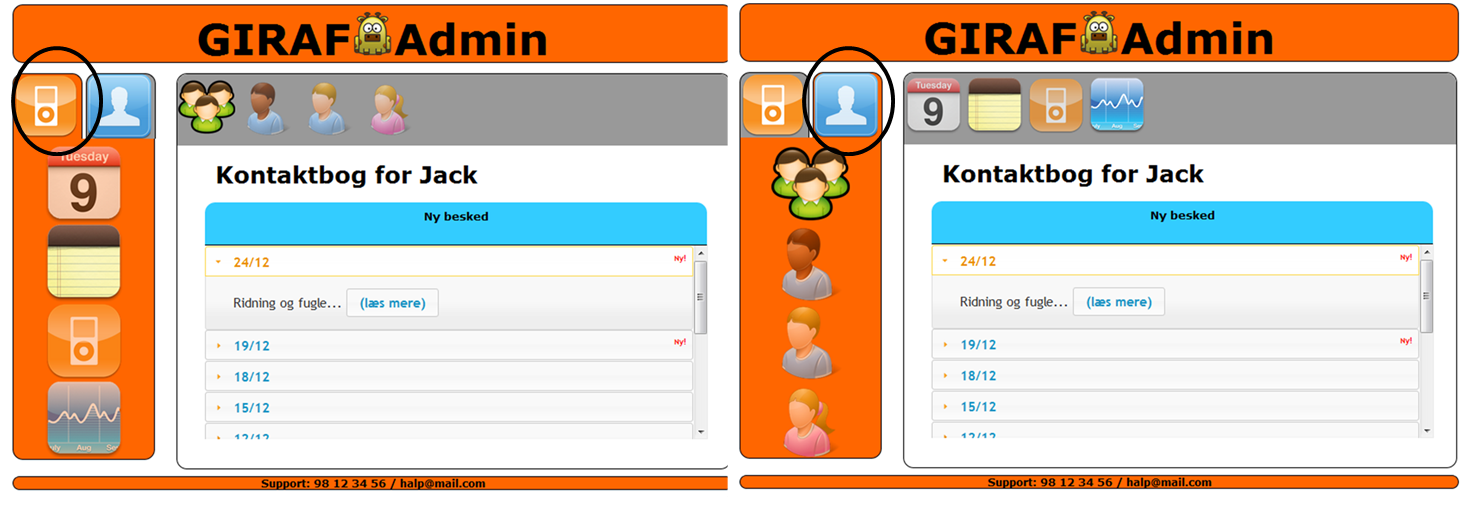
\includegraphics[width=1.00\textwidth]{img/menus.png}
	\caption{The prototype menus }
	\label{fig:menus}
\end{figure}


\subsubsection{..............Kristine kommentar.......}
her kommer tekst.

\subsection{The last paper prototype}



